%=== CHAPTER THREE (3) ===
%=== (Actual work done and contribution, including literature survey) ===

\chapter{Approach}

\section{Quantitative Trajectory Evaluation Method}
To evaluate the mapping performance, the proposed method in \cite{zhang2018tutorial} is modified to multi robot case, and employed in this work.

The previous work of CORB-SLAM in \cite{li2017corb} only provides a rough overview of the mapping result of the multi robot system, as seen in Figure \ref{fig:corbslamresult}.

In \cite{maddern2014illumination} and \cite{arroyo2016openable}, the results of the illumination variance localization are also only briefly introduced, with no quantitative results given.

In this paper, mapping results of CORB-SLAM and CORB-SLAM integrated with illumination variance are evaluated following the quantitative trajectory evaluation method proposed in \cite{zhang2018tutorial}. Quantitative evaluation results of each datasets are demonstrated in several figures and tables including contents as follows, and see Section \ref{sec:kittievaluate} as an example: 

\begin{enumerate}[1.]
	\item Ground truth trajectories of each partial sequence and the complete dataset for reference, e.g. Figure \ref{fig:kittigt}.
	\item Mapping results of each client and fused map in server end, compared with ground truth trajectories, e.g. Figure \ref{fig:kittiresults}.
	\item Four charts of quantitative results, e.g. Figure \ref{fig:kittiquanresult}, including 
	\label{enum:chartsinfo}
	\begin{enumerate}[1).]
		\item Chart of relative translation error in meter, e.g. Figure \ref{sfig:kittireltran}.
		\item Chart of relative translation error in percent, e.g. Figure \ref{sfig:kittireltranper}.
		\item Chart of relative yaw error in degree, e.g. Figure \ref{sfig:kittirelyaw}.
		\item Chart of scale error in percent, e.g. Figure \ref{sfig:kittiscaleerr}.
	\end{enumerate}
	\item A table presenting numeric results of charts in \ref{enum:chartsinfo}, e.g. Table \ref{tbl:kittiquanresult}.
	\item Charts of quantitative results of mapping each partial sequences in each client, in the same format of \ref{enum:chartsinfo}, e.g. Figure \ref{fig:kittiseq0quanresult}.
	\label{enum:clientchartinfo}
	\item A table presenting numeric results of charts in \ref{enum:clientchartinfo}, e.g. Table \ref{tbl:kittiseq0quanresult}.
	\item (if applicable) The mapping results of CORB-SLAM mapping the entire sequence without partial sequences for reference, e.g. Figure \ref{fig:kitticlientmapping}.
	\item (if applicable) Charts of quantitative results of mapping the entire sequence for reference, in the same format of \ref{enum:chartsinfo}, e.g. Figure \ref{fig:kittientirequanresult}.
	\label{enum:refchartinfo}
	\item (if applicable) A table presenting numeric results of charts in \ref{enum:refchartinfo}, e.g. Table \ref{tbl:kitticlientquanresult}.
\end{enumerate}

\begin{figure}[H]
	\centering
	\includegraphics[width=5in]{Chapter3/corbslamresult.eps}
	\caption{Mapping results of CORB-SLAM in \cite{li2017corb}.}
	\label{fig:corbslamresult} 
\end{figure}

The main task of map fusion module of multi robot SLAM server is to find relative relations including rotation and transformation matrices between client maps, based on which client maps are fused into a consist global map. Therefore, inaccurate rotation and transformation result in an inaccurate fused global map where all client maps but the one set to be the initial global map are stitched dramatically offsetting the ground truth trajectories, which therefore causes serious translation and yaw error. Therefore in charts and tables of quantitative results, three types of relative errors are selected: 

\begin{inparaenum}
	\item Relative Translation Error.

	\item Relative Translation Error in percent. 
	
	\item Relative Yaw Error.
\end{inparaenum}

Relative error computation follows the basic idea stated in \cite{zhang2018tutorial } that estimation quality can be measured by computing relative relationships between states at different times, as there is no global reference in VO systems, including global position and yaw.

Formally, given the ground truth trajectory ${\bm{X}}$ and the estimated trajectory $\hat{\bm{X}}$:

\begin{equation}
\begin{array}{lr}
{\bm{X}}=\{\bm{x}_{i}\}=\{R_i, p_i, v_i\}, & i=1,...,t.
\end{array}
\end{equation}

where, $p_i\in\Re^3$ is the position, $R_i\in{SO(3)}$ is the rotation matrix and $v_i\in\Re^{3}$ is the velocity of the system. 

 the following steps should be taken to explain and calculate relative errors:

\begin{inparaenum}[Step 1.]
	\item Given the ground truth positions$ {{{p}_i}} $ and estimated positions ${{\hat{p}}_i}$, the estimated trajectory can be aligned to the aligned estimated trajectory $\bm{\hat{X}}'$ by finding a similarity transformation $S'=\{s', {R}', {t}'\}$ that minimize:
	
	\begin{equation}
	S'=\argmin{\sum_{i=0}^{N-1}{\|{p}_i-sR{\hat{p}_i}-t\|^{2}}}.
	\end{equation}
	
	Then,
	
	\begin{equation}
	\begin{array}{lll}
		\hat{R}'_i=R'\hat{R}'_i,&  {\hat{p}'}_i=s'R'\hat{{p}}'_i+t',  & \hat{v}'_i=s'R'\hat{v}_i.
	\end{array}
	\end{equation}
	
	\item A set of K pairs of states, each of which defines a sub trajectory, need to be selected from $\hat{\bm{X}}$ by a criteria e.g. distance or duration traveled:
	
	\begin{equation}
	\begin{array}{lll}
	\bm{\xi}=\{\bm{d}_k\}_{k=0}^{K-1}, & \bm{d}_k=\{\bm{\hat{x}}_s, \bm{\hat{x}}_e\}, & e>s
	\end{array}
	\end{equation}
	
	\item Then for each $\bm{d}_k$, a relative error $\delta{\bm{d}_k}$  is calculated by:
	
	\begin{equation}
	\begin{array}{l}
	\delta{\bm{d}_k}=\{\delta{\phi}, \delta{p_k}, \delta{v_k}\}, \\
	\delta\phi_k=\angle \delta R=\angle R_e(\hat{R}'_e)^\top, \\
	\delta{p_k}=\|{p_e-\delta R_k\hat{p}'_e}\|_2, \\
	\delta{v_k}=\|v_e-\delta R_k \hat{v}'_e\|_2.
	\end{array}
	\label{eq:relerr}
	\end{equation}
	
	\item Collecting the relative errors in Equation \ref{eq:relerr} for all pairs in $\bm{\xi}$ gives:
	
	\begin{equation}
	\begin{array}{ll}
	RE_{rot}=\{\delta\phi_k\}_{k=1}^{K-1}, \\
	RE_{pos}=\{\delta p_k\}_{k=0}^{K-1}, \\
	RE_{vel}=\{\delta v_k\}_{k=0}^{K-1}, \\
	\end{array}
	\end{equation}
	
	which is illustrated in Figure \ref{fig:relerrcal}. relative translation errors in meter and percent can be extracted from $RE_{pos}$, and relative yaw errors from $RE_{rot}$.
	
	\begin{figure}[H]
		\centering
		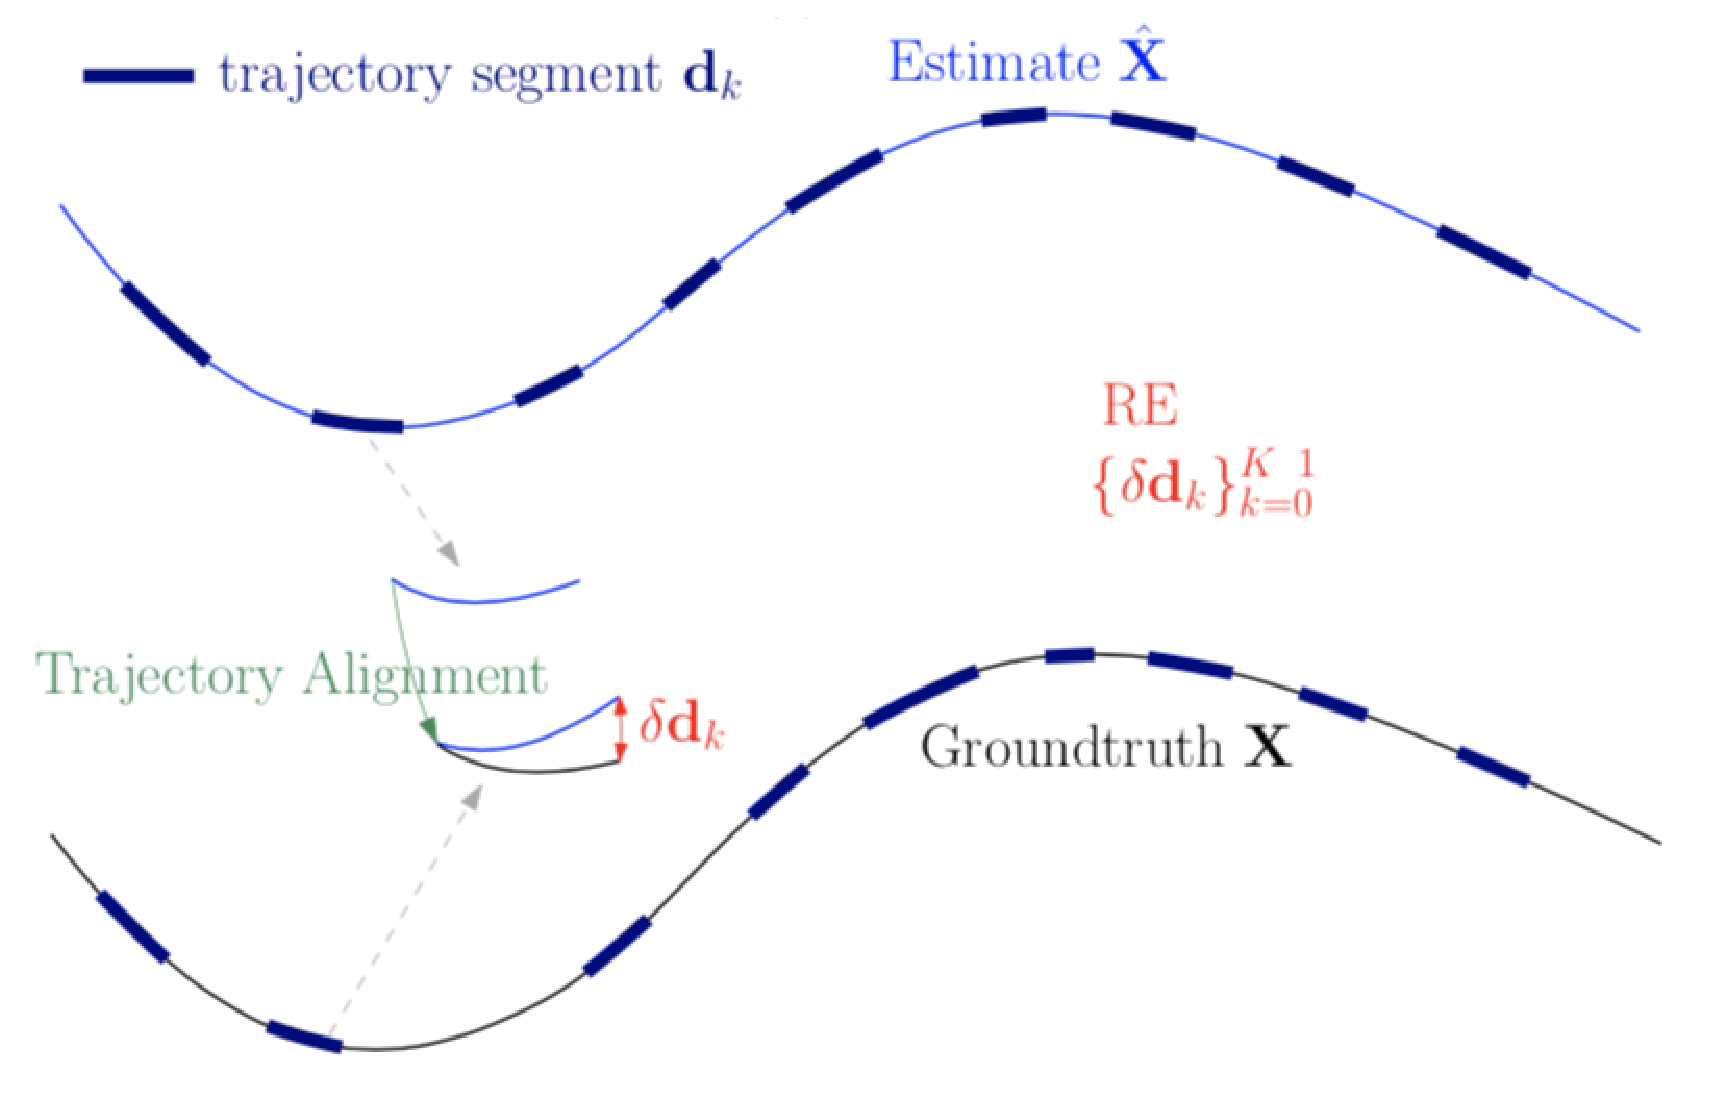
\includegraphics[width=5in]{Chapter3/relerr.eps}
		\caption{Illustration of relative error.}
		\label{fig:relerrcal} 
	\end{figure}

\end{inparaenum}

\section{CORBSLAM with Illumination Variance}

To experiment whether illumination variance method is possible to be utilized to enhance the ability of CORB-SLAM to map in different illumination conditions and seasons, it is combined into the map fusion modules of CORB-SLAM server in this work. 

In the client end, the following modifications are made:

\begin{enumerate}
	\item A new thread running in parallel is added to process the input frame to transform into illumination variance images, and extract ORB keypoints in produced images (named as \textsl{II keypoints} in this paper), as illustrated in Figure \ref{fig:keypoints}.
	\item II keypoint data is added into each frame as new member variables. And then following the CORB-SLAM methodology, only the integrated keyframes are transmitted to the server,  which are serialized and packed by boost serialization library, and transmitted through ROS service.
\end{enumerate}

\begin{figure}
	\centering
	\subfigure[Keypoints extracted from an rgb image.]{
		\begin{minipage}[t]{0.4\linewidth}
			\centering
			\includegraphics[width=2in]{Chapter3/kp_rgb.eps}
			%\caption{fig1}
		\end{minipage}
	}
	\subfigure[Keypoints extracted from an illumination variance image.]{
		\begin{minipage}[t]{0.4\linewidth}
			\centering
			\includegraphics[width=2in]{Chapter3/kp_ii.eps}
			%\caption{fig2}
		\end{minipage}
	}
	\caption{Keypoints extracted from rgb images and illumination variance images.}
	\label{fig:keypoints}
\end{figure}

Besides the above changes, the following modification are made in the server end:

\begin{enumerate}
	\item A new keydataset containing II keypoint information. 
	\item A new illumination variance localizer running in parallel with the rgb localizer. When processing the input keyframe, a new localizer thread is started if the rgb localizer returns no result. The results from rgb and illumination variance localizer are added together in this work.
	\item Since extracted II keypoint positions are not accurate as rgb keypoints, transform matrix is still trying to calculate from rgb keypoints where overlapping is detected.
\end{enumerate}





%=== END OF CHAPTER THREE ===
\newpage
